\scanpage{132}
\figure{
\begin{tikzpicture}[x=1cm,y=1cm]
\draw (.95,1.9)--(.02,.70) .. controls (.28,.91) and (.84,1.48) .. (.80,1.20) --(.31,-.12);
\draw (.32,-.12)--(1.30,1.45)--(1.05,.04);
\draw[gray] (.73,-.12) .. controls (.80,.25) and (.91,.43) .. (.98,.60);
\draw[gray!35] (1.43,.43)--(1.65,1.48);
\end{tikzpicture}}

\figure{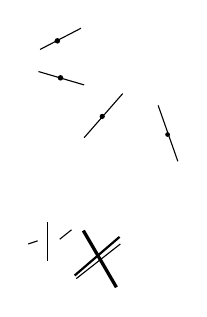
\begin{tikzpicture}[x=1cm,y=1cm]
\draw (0,1.55)--(.52,1.82); \fill (.22,1.66) circle (.035);
\draw (-.02,1.27)--(.56,1.10); \fill (.26,1.19) circle (.035);
\draw (.56,.43)--(1.05,.99); \fill (.79,.70) circle (.033);
\draw (1.5,.84)--(1.75,.13); \fill (1.62,.47) circle (.03);
\draw (-.15,-.92)--(-.03,-.88); \draw (.10,-1.13)--(.10,-.64);
\draw (.25,-.86)--(.40,-.74);
\draw[very thick] (.55,-.75)--(.97,-1.47);
\draw[thick] (.44,-1.32)--(1.01,-.83); \draw (.46,-1.36)--(1.02,-.92);
\end{tikzpicture}}

% margin note written sideways
\margin{$\begin{gathered}
x^{\unsure{2|3}}-y^{2}\\
\deleted{k(\unsure{x|x^{2}}}\\
\unsure{k|l}[\unsure{t|X}]\qquad \unsure{t|p}^{2},t^{3}\\
k[x,y]/xy
\end{gathered}$}

% letterhead
% Upside down relative to the archive number.
\begin{center}
INSTITUT\\
DES HAUTES ÉTUDES SCIENTIFIQUES\\
\rule{1cm}{0.4pt}
\end{center}

% archive sheet number: 131
